\documentclass[10pt]{article}
\usepackage[utf8]{inputenc}
\usepackage[T1]{fontenc}
\usepackage{amsmath}
\usepackage{amsfonts}
\usepackage{amssymb}
\usepackage[version=4]{mhchem}
\usepackage{stmaryrd}
\usepackage{graphicx}
\usepackage[export]{adjustbox}
\graphicspath{ {./images/} }

\title{Università di Catania 
 Corso di Laurea in Fisica 
 Compito scritto di Fisica Generale I 
 M.G. Grimaldi - S. Romano }

\author{}
\date{}


\begin{document}
\maketitle
Catania, 1 Febbraio 2023

Per la prova in itinere svolgere i problemi 1, 2, 3 (tempo 2h)

Per la prova completa svolgere i problemi 2, 3, 4, 5 (tempo 3 h).

\section{Problema n.1}
Un corpo puntiforme di massa \(m=1 \mathrm{~kg}\), inizialmente fermo all'estremo inferiore di un piano inclinato di un angolo \(\theta=30^{\circ}\) rispetto all'orizzontale, viene lanciato verso l'alto lungo il piano da un colpo di martello, che esercita su di esso un impulso di modulo \(\mathrm{J}=2 \mathrm{Ns}\). Si assuma che il contatto tra martello e corpo sia brevissimo e che lo spostamento del corpo in tale intervallo di tempo sia trascurabile. I coefficienti di attrito statico e dinamico tra il corpo e la superficie del piano sono, rispettivamente, \(\mu_{\mathrm{s}}=0.6\) e \(\mu_{\mathrm{d}}=0.2\).

a) Calcolare la lunghezza del tratto che il corpo percorre sul piano inclinato prima di fermarsi.

b) Determinare se, dopo aver raggiunto la massima quota, il corpo ricade verso il basso oppure rimane fermo.

\section{Problema n. 2}
Un proiettile di massa \(m=100 \mathrm{~g}\) viene sparato dentro un blocco di legno di massa \(M=5\) kg inizialmente fermo sul bordo di un tavolo (supposto senza attrito) a un'altezza \(\mathrm{H}=1 \mathrm{~m}\) dal pavimento (si veda la figura). Dopo l'urto, il proiettile rimane conficcato nel blocco, e il sistema blocco+proiettile cade a terra a una distanza \(\mathrm{I}=1 \mathrm{~m}\) dal punto di impatto.

a) Determinare la velocità iniziale del proiettile.

b) Si supponga ora che, dopo aver toccato il terreno, il sistema blocco+proiettile continui a strisciare per una lunghezza \(\mathrm{L}=1 \mathrm{~m}\), rallentando per poi fermarsi per effetto dell'attrito. Determinare il coefficiente di attrito dinamico tra il blocco ed il pavimento.

\begin{center}
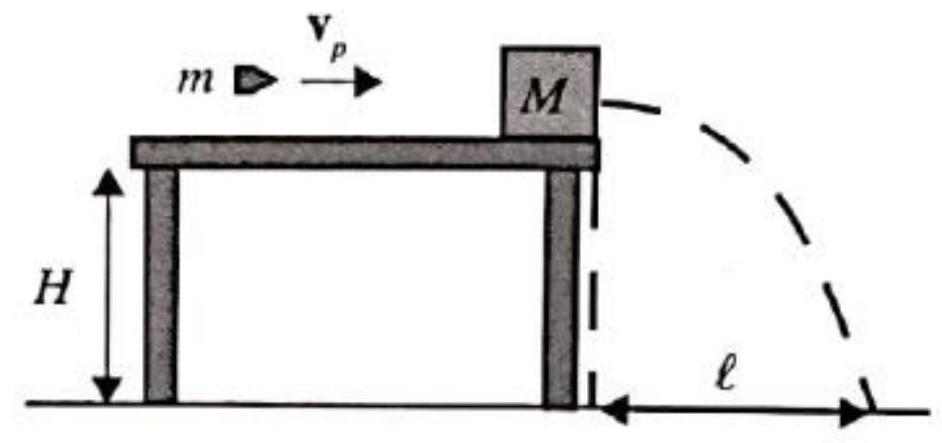
\includegraphics[max width=\textwidth]{2023_05_14_6d212a4f8f2701d0b5acg-1}
\end{center}

\section{Problema n.3}
Al bordo di un anello omogeneo di centro \(O\), raggio \(\mathrm{R}\) e massa \(M=0.765 \mathrm{~kg}\), è saldato un punto materiale \(\mathrm{P}\) di massa M. L'anello poggia su di un piano orizzontale e la congiungente PO forma un angolo di \(\pi / 6\) con la verticale passante per \(O\) (si veda la figura). Calcolare il modulo \(\mathrm{F}\) della forza (orientata come in figura) che è necessario applicare in direzione orizzontale al bordo dell'anello all'altezza di \(O\) perché il sistema si trovi in equilibrio e determinare il coefficiente di attrito minimo fra anello e piano perché tale equilibrio si mantenga.

\begin{center}
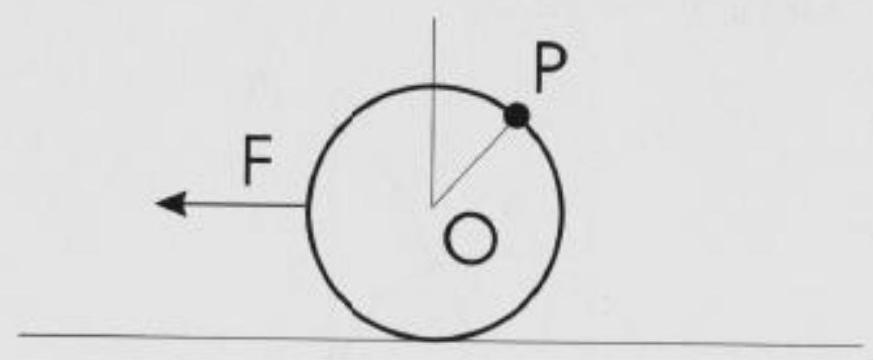
\includegraphics[max width=\textwidth]{2023_05_14_6d212a4f8f2701d0b5acg-2(1)}
\end{center}

\section{Problema n.4}
Una vasca di lunghezza \(\mathrm{L}=5 \mathrm{~m}\) è suddivisa in due parti di larghezza \(\mathrm{w}_{\mathrm{d}}=2 \mathrm{~m} \mathrm{e} \mathrm{w}_{\mathrm{s}}=1 \mathrm{~m}\) tramite una parete verticale che non arriva fino al fondo, come mostrato in figura. La vasca è riempita parzialmente di acqua (densità \(10^{3} \mathrm{~kg} / \mathrm{m}^{3}\) ) e poi, nella parte più stretta viene aggiunto dell'olio (densità \(0.84 \times 10^{3} \mathrm{~kg} / \mathrm{m}^{3}\) ). All'equilibrio, l'acqua arriva a una quota \(\mathrm{H}_{\mathrm{d}}=4 \mathrm{~m}\) nella parte destra, più larga, e a una quota \(\mathrm{H}_{\mathrm{s}}=3 \mathrm{~m}\) nella parte a sinistra, più stretta. Tutto il sistema è in aria, alla pressione atmosferica di 1 atm. Sia \(\mathrm{h}\) l'altezza della colonna d'olio sopra.

a) Calcolare il valore di \(h\).

b) Se ora si mette un blocco di legno di peso \(1000 \mathrm{~N}\) a galleggiare sull'olio, di quanto si sposta la superficie libera dell'acqua nella parte più larga della vasca?

\begin{center}
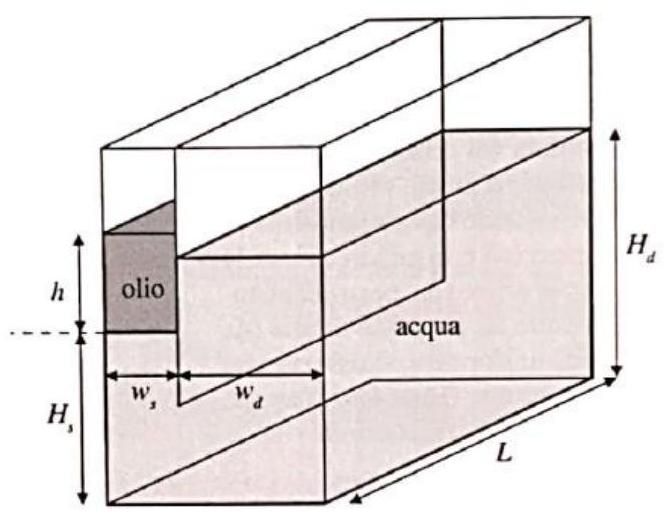
\includegraphics[max width=\textwidth]{2023_05_14_6d212a4f8f2701d0b5acg-2}
\end{center}

\section{Problema n.5}
Una mole di gas perfetto biatomico, contenuta in un cilindro munito di pistone mobile, esegue le seguenti trasformazioni: isoterma reversibile dallo stato ambiente \(A\) di pressione \(p_{A}=1\) atm e temperatura \(T_{A}=300 \mathrm{~K}\) allo stato \(B\) di pressione \(p_{B}=2 p_{A}\); adiabatica reversibile dallo stato \(B\) allo stato \(C\) di pressione \(p_{C}=p_{A}\). Infine il gas è rimesso a contatto termico con l'ambiente \(\left(T_{A}\right)\) ed esegue una rapida trasformazione a pressione costante fino a riportarsi nello stato iniziale A. Calcolare:

a) le coordinate termodinamiche degli stati B e C;

b) i calori scambiati dal gas nel ciclo;

c) il lavoro fatto sul gas nel ciclo;

d) la variazione di entropia dell'universo nel ciclo.


\end{document}